% lint-skip: 未完成ステータス（figure/table caption 未対応，人手チェック時に解消予定）
\documentclass[../../main.tex]{subfiles}
\begin{document}

\begin{flushright}
  \footnotesize\textit{【自動文字起こし・要確認】}
\end{flushright}

{\bf [解答]} $A(l,m,n)$, $B(m,n,l)$, $C(n,l,m)$ とおく ($\because$ ②)

①, ③から
\[
  \begin{cases}
    l+m+n=1 \cdots\text{④} \\
    lm+mn+nl=0 \cdots\text{⑤}
  \end{cases}
\]

(i) 点 $X\left(\dfrac{l+m+n}{3}, \dfrac{l+m+n}{3}, \dfrac{l+m+n}{3}\right)$ をとると ④から $X$ は $x+y+z=1$ 上にあり
\[ |XA|^2 = |XB|^2 = |XC|^2 = \left(\dfrac{m+n-2l}{3}\right)^2 + \left(\dfrac{n+l-2m}{3}\right)^2 + \left(\dfrac{l+m-2n}{3}\right)^2 \]
だから， $A,B,C$ は $X$ を中心とする平面 $x+y+z=1$ 上の円上にある 終

(ii) ⑤から，$\overrightarrow{OC}\cdot\overrightarrow{OA} = \overrightarrow{OB}\cdot\overrightarrow{OC} = 0$ となり，四面体$OABC$ は $\triangle OAB$ を底面とし， $OC$ を高さとする正四面体とみることができる
\begin{align}
  OA &= OB = OC = \sqrt{l^2+m^2+n^2} \\
  &= \sqrt{(l+m+n)^2 - 2(mn+nl+lm)} \\
  &= 1 \quad (\because \text{④⑤})
\end{align}
から，体積 $V$ として
\[ V = \dfrac{1}{6} = \text{const} \quad \text{終} \]

\begin{figure}[htb]
  \centering
  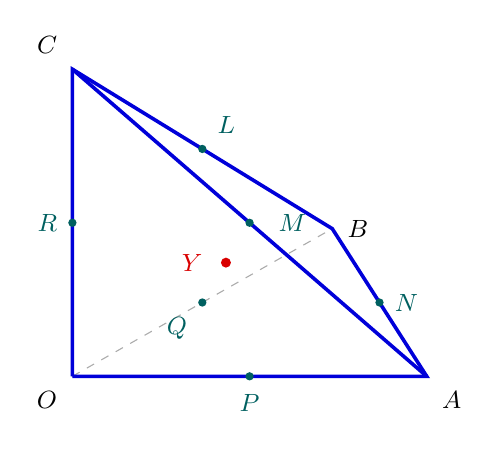
\begin{tikzpicture}[x=1.5cm, y=1.5cm,
    every node/.style={font=\small}]
    % OA, OB, OC are perpendicular in space; the drawing is a projection.
    \coordinate (O) at (0,0);
    \coordinate (A) at (3,0);
    \coordinate (B) at (2.2,1.25);
    \coordinate (C) at (0,2.6);
    \coordinate (L) at (1.1,1.925); % midpoint of BC
    \coordinate (M) at (1.5,1.3);   % midpoint of CA
    \coordinate (N) at (2.6,0.625); % midpoint of AB
    \coordinate (P) at (1.5,0);     % midpoint of OA
    \coordinate (Q) at (1.1,0.625); % midpoint of OB
    \coordinate (R) at (0,1.3);     % midpoint of OC
    \coordinate (Y) at (1.3,0.9625);
    \draw[dashed, gray!65] (O) -- (B);
    \draw[line width=1.3pt, blue!85!black]
    (O) -- (A) -- (B) -- (C) -- (O);
    \draw[line width=1.3pt, blue!85!black] (A) -- (C);
    \foreach \T in {L,M,N,P,Q,R} {
      \fill[teal!75!black] (\T) circle (1.5pt);
    }
    \fill[red!85!black] (Y) circle (1.8pt);
    \node[below left=2pt] at (O) {$O$};
    \node[below right=2pt] at (A) {$A$};
    \node[right=2pt] at (B) {$B$};
    \node[above left=2pt] at (C) {$C$};
    \node[above right=2pt, teal!75!black] at (L) {$L$};
    \node[right=7pt, teal!75!black] at (M) {$M$};
    \node[right=2pt, teal!75!black] at (N) {$N$};
    \node[below=3pt, teal!75!black] at (P) {$P$};
    \node[below left=2pt, teal!75!black] at (Q) {$Q$};
    \node[left=2pt, teal!75!black] at (R) {$R$};
    \node[left=5pt, red!85!black] at (Y) {$Y$};
  \end{tikzpicture}
  \caption{四面体 $OABC$ と6本の辺の中点 $L,M,N,P,Q,R$}
\end{figure}

$\star$ (ii) は，サラスの公式を使うと一瞬だったり，，
\[
  \left[
    \begin{array}{ccc}
      x_1 & y_1 & z_1 \\
      x_2 & y_2 & z_2 \\
      x_3 & y_3 & z_3
  \end{array} \right]
  =
  \left[
    \begin{array}{ccc}
      l & m & n \\
      m & n & l \\
      n & l & m
  \end{array} \right]
\]
\begin{align}
  V &= \dfrac{1}{6} \left| lnm + mln + nml - l^3 - n^3 - m^3 \right| \\
  &= \dfrac{1}{6} (l^2+m^2+n^2) = \dfrac{1}{6} ((l+m+n)^2-2\cdot 0) = \dfrac{1}{6}
\end{align}
※ $\left| lnm+mln+nml - l^3-m^3-n^3 \right| = (l+m+n)(l^2+m^2+n^2-lm-mn-nl)$ などを利用．

(iii) $L\left(\dfrac{m+n}{2}, \dfrac{n+l}{2}, \dfrac{l+m}{2}\right)$, $M\left(\dfrac{n+l}{2}, \dfrac{l+m}{2}, \dfrac{m+n}{2}\right)$, $N\left(\dfrac{l+m}{2}, \dfrac{m+n}{2}, \dfrac{n+l}{2}\right)$
$P\left(\dfrac{1}{2}, \dfrac{m}{2}, \dfrac{n}{2}\right)$, $Q\left(\dfrac{m}{2}, \dfrac{n}{2}, \dfrac{l}{2}\right)$, $R\left(\dfrac{n}{2}, \dfrac{l}{2}, \dfrac{m}{2}\right)$ だから，
$Y\left(\dfrac{l+m+n}{4}, \dfrac{l+m+n}{4}, \dfrac{l+m+n}{4}\right)$ とおけば
\[ |KY|^2 = \left(\dfrac{m+n-l}{4}\right)^2 + \left(\dfrac{n+l-m}{4}\right)^2 + \left(\dfrac{l+m-n}{4}\right)^2 = \text{const} \]
($K$ は $L \sim Q$ の任意の点) となり，たしかに $L \sim R$ は $Y$ を中心とする球面上にある．終

\end{document}
